\section{Uppgift 4}\label{uppgift-4}

\subsection{Instruktioner}
\begin{verbatim}
4. Skriv ett program som frågar efter åldern. Om den inmatade åldern är mindre
   än 0 så ska "Du har matat in fel ålder!" skrivas ut, annars ska "Hej, din XX
   åring!" skrivas ut. Istället för XX ska den ålder stå som skrevs in. Här är
   ett exempel på hur utskriften kan se ut, det som skrivs in från
   tangentbordet är markerat med fetstil/understrykning:

    Hur gammal är du? 28
    Hej, din 28 åring!
\end{verbatim}

\subsection{Lösning}
\subsubsection{Funktion}
För att lösa det här problemet används nästlade loopar. En yttre
\texttt{do}-loop och en inre \texttt{while}-loop.
Metoderna för ett objekt \texttt{scan} från klassen \texttt{Scanner} används
för att undersöka den inmatade texten. Den inre \texttt{while}-loopen exekveras
så länge \texttt{!scan.hasNextInt()} är sant, dvs då \texttt{scan}-objektet inte
har en integer som nästa tecken i kön för att undersökas.
\par \texttt{hasNextInt()} hoppar över tecken som används som avskiljare och
försöker sedan returnera nästa "token" i raden.
\parFör varje iteration av \texttt{while}-loopen frågas användaren om sin ålder och
\texttt{scan} hoppar över den ogiltliga inmatningen med metoden \texttt{next()}.

\begin{description}
    \item[String next()] Finds and retur:s the next complete token from this scanner.
    \item [boolean hasNextInt()] Returns true if the next token in this scanner's input can be interpreted as an int value in the default radix using the nextInt() method.
        \footnotemark
\end{description}
\footnote{\url{http://docs.oracle.com/javase/7/docs/api/java/util/Scanner.html}}

Då den inre \texttt{while}-loopen avslutas sätts variabeln \texttt{age} till 
nästa integer som står på tur i kön med \texttt{scan.nextInt()}.
\par Den yttre \texttt{do}-loopen exekveras så länge den inmatade åldern \texttt{age}
är mindre eller lika med noll. När det villkoret inte längre gäller antas \texttt{age}
hålla en giltlig ålder som skrivs ut med hjälp av \texttt{System.out.println}.

\subsubsection{Källkod}\label{uppgift-4_src}
%\begin{listing}[H]
    \inputminted[linenos]{java}{src/Lab1Uppg04.java}
    \caption{Lab1Uppg04.java}
    \label{Uppg4src}
%\end{listing}

\subsubsection{Skärmdump}
\begin{figure}[htbp]
    \centering
        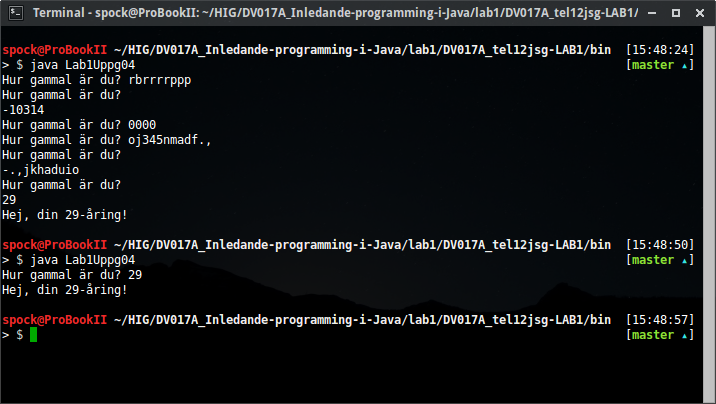
\includegraphics[width=\linewidth]{img/04.png}
    \caption{Körning av koden till Uppgift \ref{uppgift-4}}
    \label{fig:screenshot-04}
\end{figure}
